\documentclass[t,usenames,dvipsnames]{beamer}
\usetheme{Copenhagen}
\setbeamertemplate{headline}{} % remove toc from headers
\beamertemplatenavigationsymbolsempty

\usepackage{amsmath, tikz, xcolor}
\usetikzlibrary{arrows.meta, calc}

\title{Polar Coordinates}
\author{}
\date{}

\AtBeginSection[]
{
  \begin{frame}
    \frametitle{Objectives}
    \tableofcontents[currentsection]
  \end{frame}
}

\begin{document}

\begin{frame}
    \titlepage
\end{frame}

\section{Plot polar coordinates.}

\begin{frame}{Polar Coordinates}
    \begin{tabular}{p{0.4\textwidth}p{0.4\textwidth}}
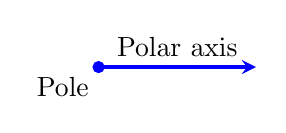
\begin{tikzpicture}
    \coordinate (O) at (0,0);
    \draw [->, >=stealth, color=blue, line width = 1.25] (O) -- (2,0) node [above, midway, black] {Polar axis}; 
    \draw [fill=blue, color=blue] (O) circle (2pt) node [below left, black] {Pole};
\end{tikzpicture}
&
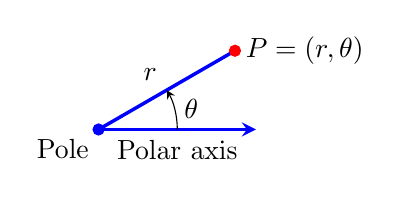
\begin{tikzpicture}
    \coordinate (O) at (0,0);
    \draw [->, >=stealth, color=blue, line width = 1.25] (O) -- (2,0) node [below, midway, black] {Polar axis}; 
    \draw [fill=blue, color=blue] (O) circle (2pt) node [below left, black] {Pole};
    \draw [-, >=stealth, color=blue, line width = 1.25] (O) -- (30:2) node [right, black] {$P=(r,\theta)$};
    \draw [color=red, fill=red] (30:2) circle (2pt);
    \draw [->,>=stealth] (0:1) arc (0:30:1) node [midway, right] {$\theta$};
    \node at (30:1) [above left] {$r$};
\end{tikzpicture}
\end{tabular}
\\[10pt]
\pause
For polar coordinates:  \newline\\
\begin{itemize}
    \item Start at the origin (pole)    \pause
    \item Go out $r$ units right ($r > 0$) or left ($r < 0$)    \pause
    \item Rotate by the amount given (\textbf{**direction**})   \pause
\end{itemize}
\vspace{10pt}

The polar coordinates of a point are $(r, \theta)$.
\end{frame}

\begin{frame}{Example 1. Plot each of the following}
\begin{minipage}{0.7\textwidth}
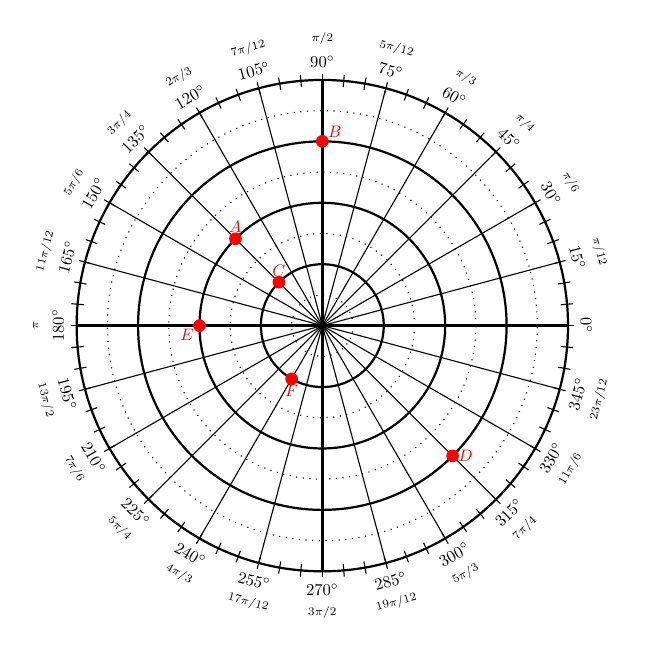
\begin{tikzpicture}[scale = 0.52, every node/.style={scale=0.6}]
    % Origin Point
    \coordinate (O) (0,0);
    % Circles
    \foreach \r in {1.5,3,...,6}
    {
        \draw[thick] (O) circle (\r cm);
    }
    
    % \foreach \r in {1.5,3,...7.5}
    % {
    %     \node at (\r, 0) [anchor=north] {\r/};
    % }
    
    \foreach \r in {0.75, 2.25,...,5.25}
    {
        \draw[dotted] (O) circle (\r cm);
    }
    
    % \node at (1.5, 0) [anchor = north west] {1};
    % \node at (3, 0) [anchor = north west] {2};
    % \node at (4.5, 0) [anchor = north west] {3};
    % \node at (6, 0) [anchor = north west] {4};
    % \node at (7.5,0) [anchor = north west] {5};
    % \foreach \r in {1.5,3,...,9}
    % {
    %     \node at (\r, 0) {\r/1.5};
    % }
    % Radial Lines
    \foreach \l in {0,15,...,360}
    {
        \draw (O) -- ++(\l:6cm);
    }
    % Thicker Radial Lines at 90 degree increments
    \foreach \l in {0,90,...,360}
    {
        \draw[very thick] (O) -- ++(\l:6cm);
    }
    % Minor Tick marks on outer circle
    \foreach \t in {0,5,...,360}
    {
        \draw (O) ++ (\t:5.85cm) -- ++(\t:0.3cm);
    }
    % Now for the fun part, the text
    % Degrees
    \node[draw=none, rotate= -90 ] at ( 0 :6.45cm) {$ 0 ^\circ$};
    \node[draw=none, rotate= -75 ] at ( 15 :6.45cm) {$ 15 ^\circ$};
    \node[draw=none, rotate= -60 ] at ( 30 :6.45cm) {$ 30 ^\circ$};
    \node[draw=none, rotate= -45 ] at ( 45 :6.45cm) {$ 45 ^\circ$};
    \node[draw=none, rotate= -30 ] at ( 60 :6.45cm) {$ 60 ^\circ$};
    \node[draw=none, rotate= -15 ] at ( 75 :6.45cm) {$ 75 ^\circ$};
    \node[draw=none, rotate= 0 ] at ( 90 :6.45cm) {$ 90 ^\circ$};
    \node[draw=none, rotate= 15 ] at ( 105 :6.45cm) {$ 105 ^\circ$};
    \node[draw=none, rotate= 30 ] at ( 120 :6.45cm) {$ 120 ^\circ$};
    \node[draw=none, rotate= 45 ] at ( 135 :6.45cm) {$ 135 ^\circ$};
    \node[draw=none, rotate= 60 ] at ( 150 :6.45cm) {$ 150 ^\circ$};
    \node[draw=none, rotate= 75 ] at ( 165 :6.45cm) {$ 165 ^\circ$};
    \node[draw=none, rotate= 90 ] at ( 180 :6.45cm) {$ 180 ^\circ$};
    \node[draw=none, rotate= 285 ] at ( 195 :6.45cm) {$ 195 ^\circ$};
    \node[draw=none, rotate= 300 ] at ( 210 :6.45cm) {$ 210 ^\circ$};
    \node[draw=none, rotate= 315 ] at ( 225 :6.45cm) {$ 225 ^\circ$};
    \node[draw=none, rotate= 330 ] at ( 240 :6.45cm) {$ 240 ^\circ$};
    \node[draw=none, rotate= 345 ] at ( 255 :6.45cm) {$ 255 ^\circ$};
    \node[draw=none, rotate= 360 ] at ( 270 :6.45cm) {$ 270 ^\circ$};
    \node[draw=none, rotate= 375 ] at ( 285 :6.45cm) {$ 285 ^\circ$};
    \node[draw=none, rotate= 390 ] at ( 300 :6.45cm) {$ 300 ^\circ$};
    \node[draw=none, rotate= 405 ] at ( 315 :6.45cm) {$ 315 ^\circ$};
    \node[draw=none, rotate= 420 ] at ( 330 :6.45cm) {$ 330 ^\circ$};
    \node[draw=none, rotate= 435 ] at ( 345 :6.45cm) {$ 345 ^\circ$};
    % Radians

    \node[draw=none, rotate= -90 ] at ( 0 :7cm) {$  $};
    \node[draw=none, rotate= -75 ] at ( 15 :7cm) {\scriptsize$ \pi/12 $};
    \node[draw=none, rotate= -60 ] at ( 30 :7cm) {\scriptsize$ \pi/6 $};
    \node[draw=none, rotate= -45 ] at ( 45 :7cm) {\scriptsize$ \pi/4 $};
    \node[draw=none, rotate= -30 ] at ( 60 :7cm) {\scriptsize$ \pi/3 $};
    \node[draw=none, rotate= -15 ] at ( 75 :7cm) {\scriptsize$ 5\pi/12 $};
    \node[draw=none, rotate= 0 ] at ( 90 :7cm) {\scriptsize$ \pi/2 $};
    \node[draw=none, rotate= 15 ] at ( 105 :7cm) {\scriptsize$ 7\pi/12 $};
    \node[draw=none, rotate= 30 ] at ( 120 :7cm) {\scriptsize$ 2\pi/3 $};
    \node[draw=none, rotate= 45 ] at ( 135 :7cm) {\scriptsize$ 3\pi/4 $};
    \node[draw=none, rotate= 60 ] at ( 150 :7cm) {\scriptsize$ 5\pi/6 $};
    \node[draw=none, rotate= 75 ] at ( 165 :7cm) {\scriptsize$ 11\pi/12 $};
    \node[draw=none, rotate= 90 ] at ( 180 :7cm) {\scriptsize$ \pi $};
    \node[draw=none, rotate= 285 ] at ( 195 :7cm) {\scriptsize$ 13\pi/2 $};
    \node[draw=none, rotate= 300 ] at ( 210 :7cm) {\scriptsize$ 7\pi/6 $};
    \node[draw=none, rotate= 315 ] at ( 225 :7cm) {\scriptsize$ 5\pi/4 $};
    \node[draw=none, rotate= 330 ] at ( 240 :7cm) {\scriptsize$ 4\pi/3 $};
    \node[draw=none, rotate= 345 ] at ( 255 :7cm) {\scriptsize$ 17\pi/12 $};
    \node[draw=none, rotate= 360 ] at ( 270 :7cm) {\scriptsize$ 3\pi/2 $};
    \node[draw=none, rotate= 375 ] at ( 285 :7cm) {\scriptsize$ 19\pi/12 $};
    \node[draw=none, rotate= 390 ] at ( 300 :7cm) {\scriptsize$ 5\pi/3 $};
    \node[draw=none, rotate= 405 ] at ( 315 :7cm) {\scriptsize$ 7\pi/4 $};
    \node[draw=none, rotate= 420 ] at ( 330 :7cm) {\scriptsize$ 11\pi/6 $};
    \node[draw=none, rotate= 435 ] at ( 345 :7cm) {\scriptsize$ 23\pi/12 $};
    
    \onslide<2->{\draw [color=red,fill=red] (135:3) circle (4pt) node [above] {$A$};}
    \onslide<4->{\draw [color=red,fill=red] (90:4.5) circle (4pt) node [above, right, yshift=0.2cm] {$B$};}
    \onslide<6->{\draw[color=red,fill=red] (135:1.5) circle (4pt) node [above] {$C$};}
    \onslide<8->{\draw[color=red,fill=red] (315:4.5) circle (4pt) node [right] {$D$};}
    \onslide<10->{\draw[color=red,fill=red] (180:3) circle (4pt) node [below, left, yshift=-0.2cm] {$E$};}
    \onslide<12->{\draw[color=red,fill=red] (240:1.5) circle (4pt) node [below] {$F$};}
\end{tikzpicture} 
\end{minipage}
\hspace{0.25cm}
\begin{minipage}{0.25\textwidth}
(a) $A\left(2, 135^\circ\right)$ \\[11pt]
\onslide<3->{(b) $B\left(-3,\frac{3\pi}{2}\right)$} \\[11pt]
\onslide<5->{(c) $C\left(-1,-\frac{\pi}{4}\right)$} \\[11pt]
\onslide<7->{(d) $D\left(3, 315^\circ\right)$} \\[11pt]
\onslide<9->{(e) $E\left(2, \pi\right)$} \\[11pt]
\onslide<11->{(f) $F\left(-1, \frac{\pi}{3}\right)$} \\
\end{minipage}
\end{frame}


\section{Convert from polar to rectangular coordinates.}

\begin{frame}{Polar to Rectangular Coordinates}

\begin{center}
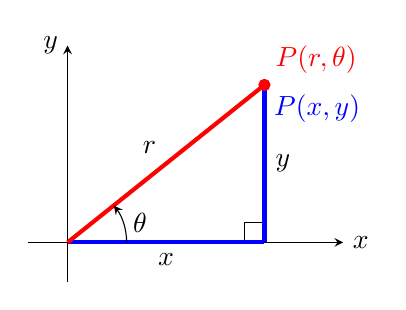
\begin{tikzpicture}
    \draw [->, >=stealth] (-0.5,0) -- (3.5,0) node [right] {$x$};
    \draw [->, >=stealth] (0,-0.5) -- (0,2.5) node [left] {$y$};
    \draw (2.5,0) rectangle +(-0.25,0.25);
    \draw [color=blue, line width = 1.5] (0,0) -- (2.5,0) node [midway, below, black] {$x$};
    \draw [color=blue, line width=1.5] (2.5,0) -- (2.5,2) node [midway, right, black] {$y$};
    \draw [color=red, line width=1.5] (0,0) -- (2.5,2) node [above right] {$P(r,\theta)$};
    \draw [color=red, fill=red] (2.5,2) circle (2pt);
    \node at (2.5,2) [below right, blue] {$P(x, y)$};
    \node at (1.25, 1) [above left] {$r$};
    \draw [->, >=stealth] (0:0.75) arc (0:38.5:0.75) node [midway, right] {$\theta$};
\end{tikzpicture}
\end{center}
\pause

\begin{align*}
    \onslide<2->{\cos\theta = \frac{x}{r} \qquad & \qquad \sin\theta = \frac{y}{r}} \\[11pt]
    \onslide<3->{x = r\cos \theta \qquad & \qquad y = r\sin \theta}   \\
\end{align*}
\end{frame}

\begin{frame}{Example 2}
Convert each to rectangular coordinates.    \newline\\
(a) \quad $\left(2, 270^\circ\right)$
\begin{align*}
    \onslide<2->{x=2\cos270^\circ \quad & \quad y = 2\sin270^\circ} \\[10pt]
    \onslide<3->{x=2(0) \quad & \quad y = 2(-1)} \\[10pt]
    \onslide<4->{x=0 \quad & y = -2} \\
\end{align*}
\onslide<5->{\[(0,2)\]}
\end{frame}

\begin{frame}{Example 2}
    \begin{center}
    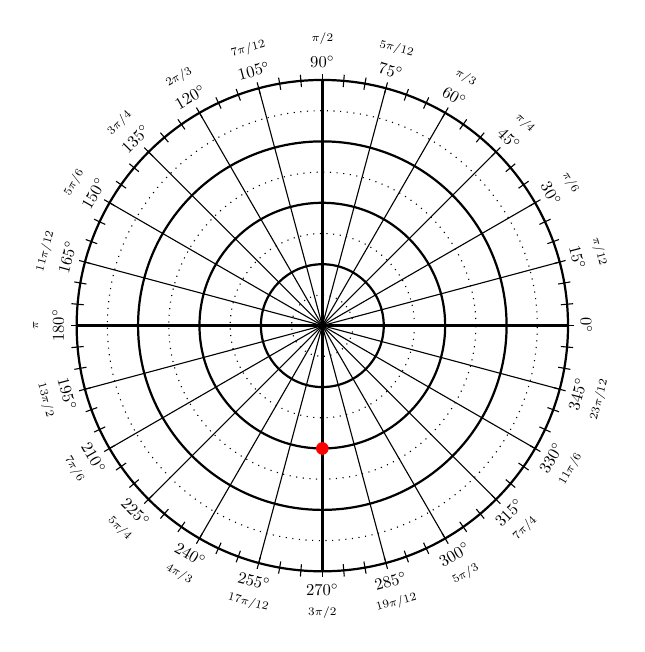
\begin{tikzpicture}[scale = 0.52, every node/.style={scale=0.6}]
    % Origin Point
    \coordinate (O) (0,0);
    % Circles
    \foreach \r in {1.5,3,...,6}
    {
        \draw[thick] (O) circle (\r cm);
    }
    
    % \foreach \r in {1.5,3,...7.5}
    % {
    %     \node at (\r, 0) [anchor=north] {\r/};
    % }
    
    \foreach \r in {0.75, 2.25,...,5.25}
    {
        \draw[dotted] (O) circle (\r cm);
    }
    
    % \node at (1.5, 0) [anchor = north west] {1};
    % \node at (3, 0) [anchor = north west] {2};
    % \node at (4.5, 0) [anchor = north west] {3};
    % \node at (6, 0) [anchor = north west] {4};
    % \node at (7.5,0) [anchor = north west] {5};
    % \foreach \r in {1.5,3,...,9}
    % {
    %     \node at (\r, 0) {\r/1.5};
    % }
    % Radial Lines
    \foreach \l in {0,15,...,360}
    {
        \draw (O) -- ++(\l:6cm);
    }
    % Thicker Radial Lines at 90 degree increments
    \foreach \l in {0,90,...,360}
    {
        \draw[very thick] (O) -- ++(\l:6cm);
    }
    % Minor Tick marks on outer circle
    \foreach \t in {0,5,...,360}
    {
        \draw (O) ++ (\t:5.85cm) -- ++(\t:0.3cm);
    }
    % Now for the fun part, the text
    % Degrees
    \node[draw=none, rotate= -90 ] at ( 0 :6.45cm) {$ 0 ^\circ$};
    \node[draw=none, rotate= -75 ] at ( 15 :6.45cm) {$ 15 ^\circ$};
    \node[draw=none, rotate= -60 ] at ( 30 :6.45cm) {$ 30 ^\circ$};
    \node[draw=none, rotate= -45 ] at ( 45 :6.45cm) {$ 45 ^\circ$};
    \node[draw=none, rotate= -30 ] at ( 60 :6.45cm) {$ 60 ^\circ$};
    \node[draw=none, rotate= -15 ] at ( 75 :6.45cm) {$ 75 ^\circ$};
    \node[draw=none, rotate= 0 ] at ( 90 :6.45cm) {$ 90 ^\circ$};
    \node[draw=none, rotate= 15 ] at ( 105 :6.45cm) {$ 105 ^\circ$};
    \node[draw=none, rotate= 30 ] at ( 120 :6.45cm) {$ 120 ^\circ$};
    \node[draw=none, rotate= 45 ] at ( 135 :6.45cm) {$ 135 ^\circ$};
    \node[draw=none, rotate= 60 ] at ( 150 :6.45cm) {$ 150 ^\circ$};
    \node[draw=none, rotate= 75 ] at ( 165 :6.45cm) {$ 165 ^\circ$};
    \node[draw=none, rotate= 90 ] at ( 180 :6.45cm) {$ 180 ^\circ$};
    \node[draw=none, rotate= 285 ] at ( 195 :6.45cm) {$ 195 ^\circ$};
    \node[draw=none, rotate= 300 ] at ( 210 :6.45cm) {$ 210 ^\circ$};
    \node[draw=none, rotate= 315 ] at ( 225 :6.45cm) {$ 225 ^\circ$};
    \node[draw=none, rotate= 330 ] at ( 240 :6.45cm) {$ 240 ^\circ$};
    \node[draw=none, rotate= 345 ] at ( 255 :6.45cm) {$ 255 ^\circ$};
    \node[draw=none, rotate= 360 ] at ( 270 :6.45cm) {$ 270 ^\circ$};
    \node[draw=none, rotate= 375 ] at ( 285 :6.45cm) {$ 285 ^\circ$};
    \node[draw=none, rotate= 390 ] at ( 300 :6.45cm) {$ 300 ^\circ$};
    \node[draw=none, rotate= 405 ] at ( 315 :6.45cm) {$ 315 ^\circ$};
    \node[draw=none, rotate= 420 ] at ( 330 :6.45cm) {$ 330 ^\circ$};
    \node[draw=none, rotate= 435 ] at ( 345 :6.45cm) {$ 345 ^\circ$};
    % Radians

    \node[draw=none, rotate= -90 ] at ( 0 :7cm) {$  $};
    \node[draw=none, rotate= -75 ] at ( 15 :7cm) {\scriptsize$ \pi/12 $};
    \node[draw=none, rotate= -60 ] at ( 30 :7cm) {\scriptsize$ \pi/6 $};
    \node[draw=none, rotate= -45 ] at ( 45 :7cm) {\scriptsize$ \pi/4 $};
    \node[draw=none, rotate= -30 ] at ( 60 :7cm) {\scriptsize$ \pi/3 $};
    \node[draw=none, rotate= -15 ] at ( 75 :7cm) {\scriptsize$ 5\pi/12 $};
    \node[draw=none, rotate= 0 ] at ( 90 :7cm) {\scriptsize$ \pi/2 $};
    \node[draw=none, rotate= 15 ] at ( 105 :7cm) {\scriptsize$ 7\pi/12 $};
    \node[draw=none, rotate= 30 ] at ( 120 :7cm) {\scriptsize$ 2\pi/3 $};
    \node[draw=none, rotate= 45 ] at ( 135 :7cm) {\scriptsize$ 3\pi/4 $};
    \node[draw=none, rotate= 60 ] at ( 150 :7cm) {\scriptsize$ 5\pi/6 $};
    \node[draw=none, rotate= 75 ] at ( 165 :7cm) {\scriptsize$ 11\pi/12 $};
    \node[draw=none, rotate= 90 ] at ( 180 :7cm) {\scriptsize$ \pi $};
    \node[draw=none, rotate= 285 ] at ( 195 :7cm) {\scriptsize$ 13\pi/2 $};
    \node[draw=none, rotate= 300 ] at ( 210 :7cm) {\scriptsize$ 7\pi/6 $};
    \node[draw=none, rotate= 315 ] at ( 225 :7cm) {\scriptsize$ 5\pi/4 $};
    \node[draw=none, rotate= 330 ] at ( 240 :7cm) {\scriptsize$ 4\pi/3 $};
    \node[draw=none, rotate= 345 ] at ( 255 :7cm) {\scriptsize$ 17\pi/12 $};
    \node[draw=none, rotate= 360 ] at ( 270 :7cm) {\scriptsize$ 3\pi/2 $};
    \node[draw=none, rotate= 375 ] at ( 285 :7cm) {\scriptsize$ 19\pi/12 $};
    \node[draw=none, rotate= 390 ] at ( 300 :7cm) {\scriptsize$ 5\pi/3 $};
    \node[draw=none, rotate= 405 ] at ( 315 :7cm) {\scriptsize$ 7\pi/4 $};
    \node[draw=none, rotate= 420 ] at ( 330 :7cm) {\scriptsize$ 11\pi/6 $};
    \node[draw=none, rotate= 435 ] at ( 345 :7cm) {\scriptsize$ 23\pi/12 $};
    \draw [color=red,fill=red] (270:3) circle (4pt);
    \end{tikzpicture}
    \end{center}
\end{frame}

\begin{frame}{Example 2}
\begin{center}
\begin{tikzpicture}[scale=0.52]
    \draw [<->,>=stealth,very thick] (-6,0) -- (6,0) node [right] {$x$};
    \draw [<->,>=stealth,very thick] (0,-6) -- (0,6) node [right] {$y$};
    \foreach \x in {-4.5,-3,...,4.5}
    \draw [thick] (\x,0.2) -- (\x,-0.2);
    \foreach \y in {-4.5,-3,...,4.5}
    \draw [thick] (0.2,\y) -- (-0.2,\y);
    \draw [color=red,fill=red] (0,-3) circle (4pt);
\end{tikzpicture}
\end{center}
\end{frame}

\begin{frame}{Example 2}
(b) \quad $\left(-8, \frac{\pi}{3}\right)$
\begin{align*}
    \onslide<2->{x = -8\cos\left(\frac{\pi}{3}\right) \quad & \quad y = -8\sin\left(\frac{\pi}{3}\right)} \\[10pt]
    \onslide<3->{x = -8\left(\frac{1}{2}\right) \quad & \quad y = -8\left(\frac{\sqrt{3}}{2}\right)} \\[10pt]
    \onslide<4->{x = -4 \quad & \quad y = -4\sqrt{3}}
\end{align*}
\onslide<5->{\[\left(-4, -4\sqrt{3}\right) \]}
\end{frame}

\section{Convert from rectangular to polar coordinates.}

\begin{frame}{Rectangular to Polar}
\begin{center}
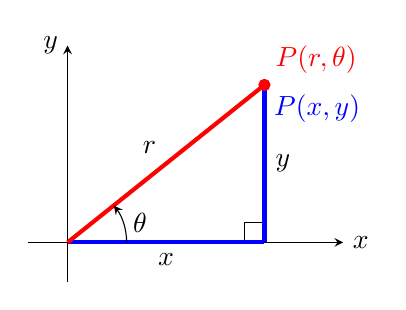
\begin{tikzpicture}
    \draw [->, >=stealth] (-0.5,0) -- (3.5,0) node [right] {$x$};
    \draw [->, >=stealth] (0,-0.5) -- (0,2.5) node [left] {$y$};
    \draw (2.5,0) rectangle +(-0.25,0.25);
    \draw [color=blue, line width = 1.5] (0,0) -- (2.5,0) node [midway, below, black] {$x$};
    \draw [color=blue, line width=1.5] (2.5,0) -- (2.5,2) node [midway, right, black] {$y$};
    \draw [color=red, line width=1.5] (0,0) -- (2.5,2) node [above right] {$P(r,\theta)$};
    \draw [color=red, fill=red] (2.5,2) circle (2pt);
    \node at (2.5,2) [below right, blue] {$P(x, y)$};
    \node at (1.25, 1) [above left] {$r$};
    \draw [->, >=stealth] (0:0.75) arc (0:38.5:0.75) node [midway, right] {$\theta$};
\end{tikzpicture}
\end{center}
\pause
\[
r = \sqrt{x^2+y^2} \qquad \onslide<3->{\theta' = \tan^{-1}\left| \frac{y}{x} \right|}
\]
\vspace{8pt}
\onslide<4->{where $\theta '$ is the \underline{reference angle} used to find the total angle rotated, $\theta$.}
\end{frame}

\begin{frame}{Example 3}
Convert each of the following to polar coordinates. \newline\\
(a) \quad $\left(-1, \sqrt{3}\right)$   \newline\\
\begin{minipage}{0.5\textwidth}
\begin{tikzpicture}[scale=0.9]
\draw[<->,>=stealth] (-2.5,0) -- (2.5,0) node [right] {$x$};
\draw[<->,>=stealth] (0,-2.5) -- (0,2.5) node [above] {$y$};
\coordinate (A) at (-1,1.73);
\draw[fill=black] (A) circle (2pt);
\onslide<2->{\draw (0,0) -- (A) -- node [left] {\scriptsize $\sqrt{3}$} (-1,0) -- node [below] {\scriptsize $-1$} cycle;}
\onslide<4->{\node at (-0.3,0.15) {\scriptsize $\theta'$};}
\onslide<4->{\node at (120:1) [above, xshift=0.1cm] {\scriptsize 2};}
\onslide<6->{\node at (-0.3,0.15) [color=white,fill=white] {};}
\onslide<6->{\node at (-0.35,0.15) {\scriptsize $60^\circ$};}
\onslide<7->{\draw[->,>=stealth,color=red] (0.75,0) arc (0:120:0.75) node [above right, xshift=0.3cm] {\scriptsize $120^\circ$};}
\end{tikzpicture}
\end{minipage}
\hspace{-0.5cm}
\begin{minipage}{0.5\textwidth}
\begin{align*}
    \onslide<3->{r &= \sqrt{1^2 + (\sqrt{3})^2} = \sqrt{4} = 2}  \\[8pt]
    \onslide<5->{\theta' &= \tan^{-1}\left|\frac{\sqrt{3}}{-1}\right| = 60^\circ}    \\[8pt]
    \onslide<7->{\theta &= 120^\circ} \\[8pt]
    & \onslide<8->{\left(2, 120^\circ\right)} \\
\end{align*}
\end{minipage}
\end{frame}

\begin{frame}{Example 3}
(b) \quad $(1, -1)$ \newline\\
\begin{minipage}{0.4\textwidth}
\begin{tikzpicture}[scale=0.8]
\draw[<->,>=stealth] (-2.5,0) -- (2.5,0) node [right] {$x$};
\draw[<->,>=stealth] (0,-2.5) -- (0,2.5) node [above] {$y$};
\coordinate (A) at (1.75,-1.75);
\draw [fill=black] (A) circle (2pt);
\onslide<2->{\draw (0,0) -- (A) -- node [right] {\scriptsize $-1$} (1.75,0) -- node [above] {\scriptsize 1} cycle;}
\onslide<4->{\node at (0.5,-0.2) {\scriptsize $\theta'$};}
\onslide<4->{\node at (315:1) [below, yshift=-0.1cm] {\scriptsize $\sqrt{2}$};}
\onslide<6->{\node at (0.5,-0.2) [color=white,fill=white] {};}
\onslide<6->{\node at (0.6,-0.2) {\scriptsize $45^\circ$};}
\onslide<7->{\draw[->,>=stealth,color=red] (0.75,0) arc (0:315:0.75) node [midway, above left] {\scriptsize $315^\circ$};}
\end{tikzpicture}
\end{minipage}
\hspace{0.5cm}
\begin{minipage}{0.5\textwidth}
\begin{align*}
    \onslide<3->{r &= \sqrt{1^2 + 1^2} = \sqrt{2}}  \\[8pt]
    \onslide<5->{\theta' &= \tan^{-1}\left|\frac{-1}{1}\right| = 45^\circ}    \\[8pt]
    \onslide<7->{\theta &= 315^\circ} \\[8pt]
    & \onslide<8->{\left(\sqrt{2}, 315^\circ\right)} \\
\end{align*}
\end{minipage}
\end{frame}


\section{Convert rectangular and polar equations.}

\begin{frame}{Rectangular and Polar Equations}
We can use the relationship between rectangular and polar coordinates to convert equations of one form to the other.  \newline\\  \pause

\begin{tabular}{p{0.4\textwidth}p{0.4\textwidth}}
    \onslide<2->{$x = r\cos \theta$}  & \onslide<3->{$x^2 + y^2 = r^2$}  \\
    \onslide<2->{$y = r\sin\theta$}   & \onslide<3->{$\tan\theta = \dfrac{y}{x}$}  \\ 
\end{tabular}
\end{frame}

\begin{frame}{Example 4}
    Convert each to polar equations.    \newline\\
(a) \quad $x + y = 5$ 
\begin{align*}
    \onslide<2->{{\color{red}x}+{\color{blue}y} &= 5} \\[8pt]
    \onslide<3->{{\color{red}r\cos\theta} + {\color{blue}r\sin\theta} &= 5} \\[8pt]
    \onslide<4->{r\left(\cos\theta + \sin\theta\right) &= 5} \\[8pt]
    \onslide<5->{r &= \frac{5}{\cos\theta + \sin\theta}} \\
\end{align*}
\end{frame}

\begin{frame}{Example 4}
(b) \quad $3x-y=6$
\begin{align*}
    \onslide<2->{3{\color{red}x}-{\color{blue}y} &= 6} \\[8pt]
    \onslide<3->{3{\color{red}r\cos\theta} - {\color{blue}r\sin\theta} &= 6} \\[8pt]
    \onslide<4->{r\left(3\cos\theta - \sin\theta \right) &= 6} \\[8pt]
    \onslide<5->{r &= \frac{6}{3\cos\theta - \sin\theta}}
\end{align*}
\end{frame}


\begin{frame}{Example 5}
Convert each of the following to rectangular equations. \newline\\
(a) \quad $r = 5$
\begin{align*}
    \onslide<2->{r &= 5} \\[8pt]
    \onslide<3->{r^2 &= 25} \\[8pt]
    \onslide<4->{x^2+y^2 &= 25} 
\end{align*}
\end{frame}

\begin{frame}{Example 5}
(b) \quad $\theta = \dfrac{\pi}{4}$
\begin{align*}
    \onslide<2->{\theta &= \frac{\pi}{4}} \\[8pt]
    \onslide<3->{\tan \theta &= \tan\left(\frac{\pi}{4}\right)} \\[8pt]
    \onslide<4->{\frac{y}{x} &= 1} \\[8pt]
    \onslide<5->{y &= x} \\
\end{align*}
\end{frame}

\begin{frame}{Example 5}
(c) \quad $r = 3\csc\theta$
\begin{align*}
    \onslide<2->{r &= 3\csc\theta} \\[8pt]
    \onslide<3->{r &= 3\left(\frac{1}{\sin\theta}\right)} \\[8pt]
    \onslide<4->{r &= \frac{3}{\sin\theta}} \\[8pt]
    \onslide<5->{r\sin\theta &= 3} \\[8pt]
    \onslide<6->{y &= 3} \\
\end{align*}
\end{frame}

\begin{frame}{Example 5}
(d) \quad $r = -6\cos\theta$
\begin{align*}
    \onslide<2->{r &= -6\cos\theta} \\[8pt]
    \onslide<3->{r^2 &= -6{\color{red}r\cos\theta}} \\[8pt]
    \onslide<4->{x^2 + y^2 &= -6x} \\[8pt]
    \onslide<5->{x^2+6x+y^2 &= 0} \\
\end{align*}
\end{frame}

\end{document}
